\chapter{Probleemanalyse}
\label{hoofdstuk:probleemanalyse}
\section{De aanleiding}
Deze opdracht is ontstaan vanuit de finance afdeling in het afgelopen jaar. Deze handelt registrerend en controlerend ten behoeve van de geld-goederenstroom. De intern beschikkende afdelingen –-- inkoop en verkoop --– werken nauw samen met finance voor de bewaking en afdekking van valuta-, rente- en koersrisico (hierna als afkorting: FX). Het management en de afdeling finance hebben samen een voorkeur voor een formeel vastgelegd beleid voor het geldmiddelenbeheer en zochten hiervoor een passende afstudeerder. Daarnaast was de verouderde AOIB toe aan vernieuwing.

\section{Probleemomschrijving}
\label{beschr:problemen}
De AOIB bij Seafood Connection is in lichte mate verouderd, concreet betekent dit dat sinds de laatste update er nieuwe afdelingen zijn ontstaan, er nieuwe functies zijn gecreëerd of zijn veranderd, en dat het organogram veranderd is. Het bedrijf is sinds de laatste update verdubbeld qua omzet en personeel. Een update is dus hoognodig om te voorkomen dat de vastgelegde AOIB niet overeenkomt met de werkelijkheid. 
Het vastleggen van de AOIB is niet meer dan een momentopname van de organisatie, het hebben van een goed omschreven AO leidt dus niet automatisch tot interne beheersing. Het denken over, en vastleggen van deze AOIB kan wel enige bewustwording stimuleren zodat er kritisch gaat nagedacht worden over hoe de organisatie wordt ingericht. \citep{bivpraktijk}

Juist door deze verouderde AO is er een verschil tussen de daadwerkelijke bedrijfsprocessen en de formele vastlegging hiervan. Het knelpunt hier is de vastlegging van de organisatorische maatregelen rond de financiële geldstromen. Zoals eerder beschreven in paragraaf \ref{beschr:activiteiten} haalt Seafood Connection haar bestaansgrond uit het feit dat er op grote schaal wordt ingekocht en verkocht op een internationale markt. De geld-goederenstroom is een cruciaal deel van de bedrijfsvoering die op het moment niet uitgebreid en doordacht is vastgelegd. \citep{aoibsfc}

De organisatorische maatregelen rond de financiële geldstromen komen voort uit de AOIB, de aflegging van het beleid over financiële geldstromen is dus onlosmakelijk van de administratieve organisatie. 

Momenteel is er nog niet een vastgelegd document omtrent de \textit{treasury} dat aansluit op het beleid rondom geldzaken. Treasurybeleid is de manier waarop een onderneming haar \textit{treasures} (of ook: schatten) beheert. De praktische invulling van het treaurybeleid wordt omschreven in het door het management opgestelde treasury statuut. 
Dit statuut is \textbf{intern} gericht door in kaart te brengen hoe de verschillende processen rond de financiële beheersing horen te functioneren, er wordt bijvoorbeeld beschreven wie welke functie heeft in het geld-goederenproces en welke controles daarop uitgevoerd worden. \\
Ook is het statuut \textbf{extern} gericht aan stakeholders door de verantwoording die wordt afgelegd, door het management, over het geldbeheer. \citep{jans}

In deze en volgende rapportage wordt de volgende definitie gehanteerd voor de term treasury statuut: 

\begin{displayquote}
Het treasury statuut is een door het management opgesteld rapport waarin de bevoegdheden, verantwoordelijkheden, toezichtmaatregelen, de sturing, en beheersing geformuleerd worden ten aanzien van financiële vermogenswaarden, financiële geldstromen, financiële posities en de hieraan verbonden risico’s. \\
\citep{jans,buunk} \label{def:treasury}
\end{displayquote}
\noindent
Zie ook \hyperlink{bij:treasury}{bijlage 1} voor een overzichtelijke uitwerking van het begrip treasury statuut.

\bigskip
De treasuryfunctie is een essentieel deel van alle primaire processen bij Seafood Connection door de grote aanwezigheid van vreemde valuta in zowel het inkoop- als verkoopproces. In figuur \ref{fig:primairproces} is te zien hoe de primaire processen verband houden met elkaar. Enkele communicatiestromen zijn hier ook weergegeven, namelijk de inkopers die voor het betalen van een levering in een andere valuta aan de finance-afdeling het verzoek sturen om euro's te verkopen voor bijvoorbeeld dollars. De verkopers vragen aan de finance-afdeling of zij vreemde valuta willen inkopen om de brutomarge vast te zetten.

\begin{figure}[!hb]
    \centering
    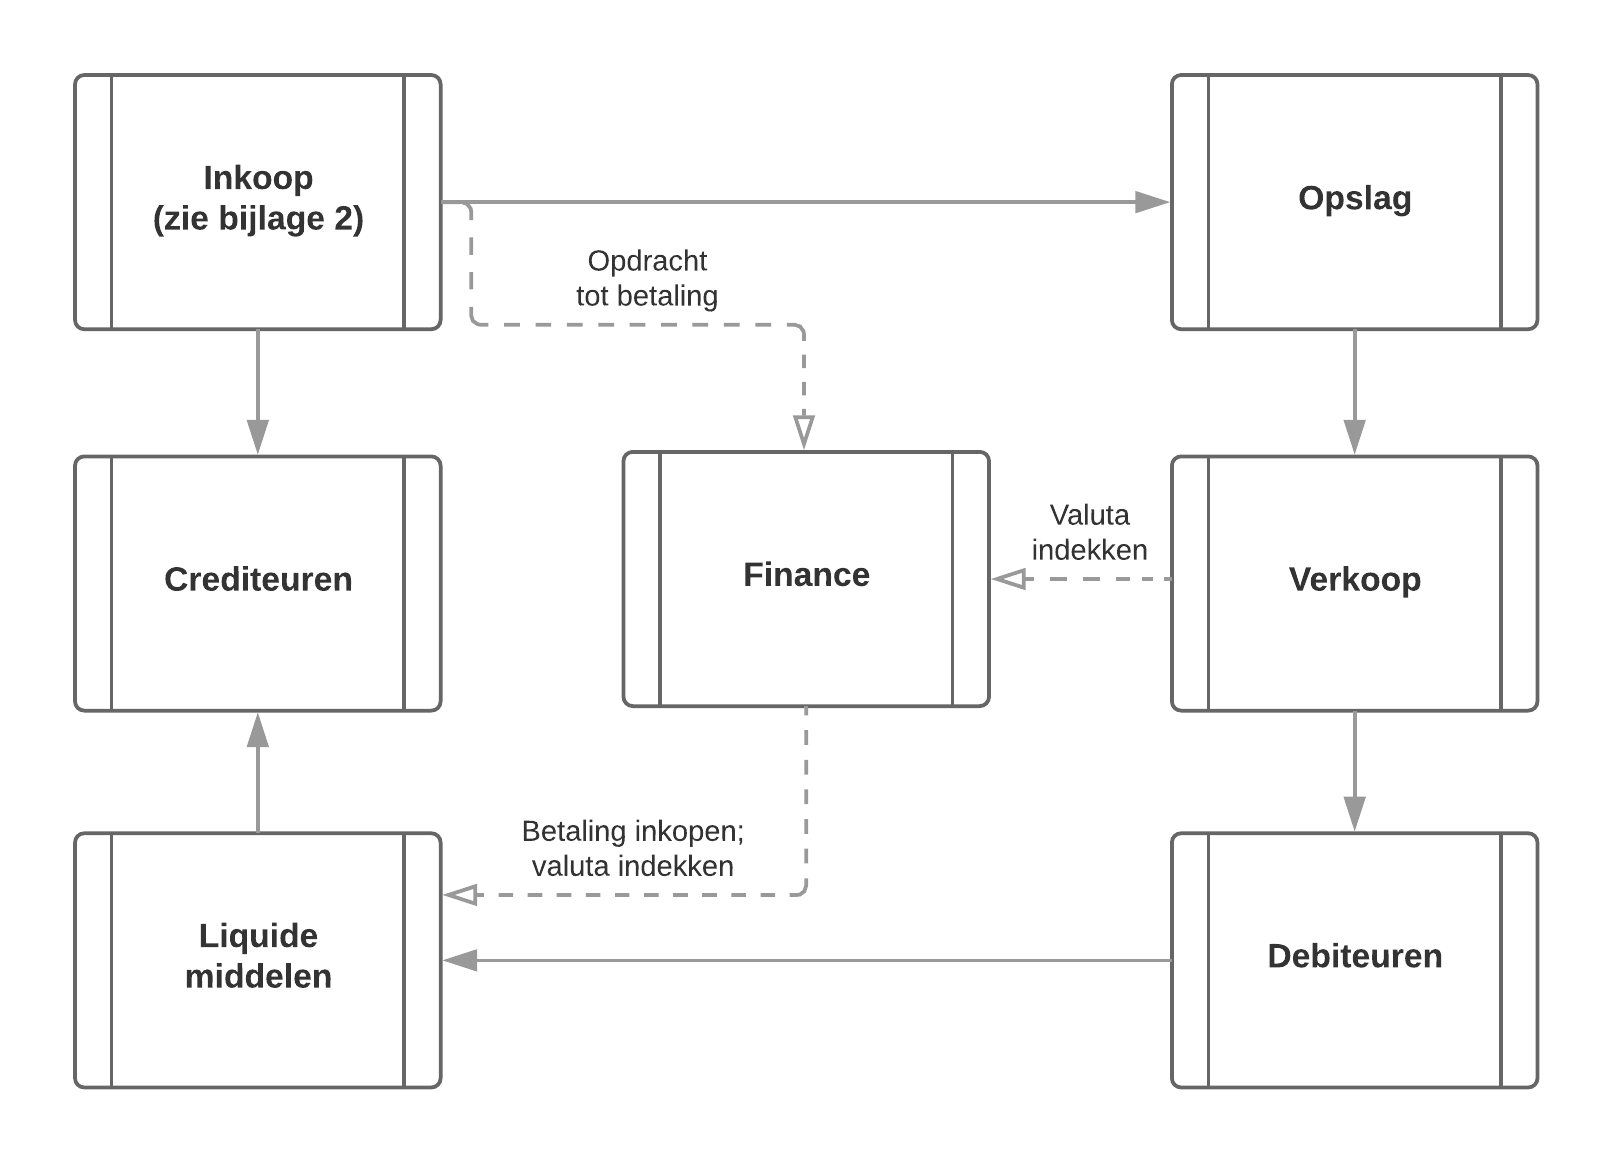
\includegraphics[width=0.78\textwidth]{primairproces}
    \caption{Globaal overzicht van de primaire processen}
    \label{fig:primairproces}
\end{figure}

Samenvattend worden de huidige bestaande organisatorische maatregelen en processen in kaart gebracht. Daarnaast is het management van SFC bewust dat er op een navolgbare en verantwoordelijke manier omgegaan moet worden met financiële middelen; immers handelt het bedrijf met een uitputbare hoeveelheid vreemde valuta en is er een hoge mate van liquiditeit vereist om het bestaan van het bedrijf in de toekomst te kunnen garanderen. Het treasury statuut is onlosmakelijk verbonden met de AOIB, het is daarom noodzakelijk dit product pas wordt opgesteld wanneer de AO weer aansluit op de werkelijkheid \citep{watisonderzoek,buunk,financiering}.

\subsection{De doelstelling}
Zoals hiervoor beschreven wordt de bestaande AOIB bijgewerkt waarbij vervolgens een zogenaamde treasury statuut wordt opgesteld (zie paragraaf \ref{def:treasury}). Het statuut komt voort uit de AOIB. 
Om deze twee producten op te leveren wordt eerst het interne betrouwbaarheidssysteem onder de loep genomen waarbij vooral gekeken wordt naar de goede en slechte aspecten van de organisatorische inrichting. De geüpdatete AOIB en het treasury statuut zijn 'deliverables', dat wil zeggen dat zij voortvloeien uit de opdracht zelf. In het treasury statuut legt het management verantwoording af over het kas- en geldmiddelenbeheer en dus ook over hoe FX-risico wordt bestreden. Deze aflegging van de verantwoording over de financiële middelen moet in lijn zijn met de getroffen, organisatorische maatregelen en de manier waarop het management idealistisch de geldstromen bewaakt en monitort. Het management geeft zelf aan dat het opstellen van dit statuut een hoognodig deel is van het onderzoek, aangezien er al een bestaande AO aanwezig is en dat het kasmanagement, hoewel grotendeels geautomatiseerd, nog niet formeel is vastgelegd. Bij de uitwerking van de update van de AO wordt door de organisatorische veranderingen (beschreven in paragraaf \ref{beschr:problemen}) ook rekening gehouden met nieuwe afdelingen, veranderde afdelingen, nieuwe organisatiestructuren, afdelingen die gericht zijn op nieuwe producten en nieuwe markten.

Bij deze ontwerpende opdracht is aan het einde van het afstudeertraject de AOIB bijgewerkt en in brede zin in kaart gebracht. Nadenken over de structuren en maatregelen, zoals dat in een AO-beschrijving gebeurt, is voor veel bedrijven belangrijk om niet alleen te kunnen groeien in de toekomst, maar ook om het bestaan van de onderneming enigszins te kunnen garanderen en om te toetsen of er niet ongeoorloofd middelen uit de onderneming wegvloeien.

Belangrijk om in gedachten te houden bij deze opdracht is dat deze opdracht zowel intern als extern is gericht. Intern wordt verslag gedaan over de administratieve organisatie en deze wordt geüpdatet. Het is dus niet de bedoeling dat derden dit document voor handen krijgen. Het op te stellen treasury statuut is echter wel bedoeld voor derden want het is een verantwoording van het management over hoe er wordt omgegaan met financiële middelen. Stakeholders kunnen met dit document helderheid krijgen op het valutabeheer van de onderneming. Bij de uitwerking van deze twee deelproducten moet de bedoelde doelgroep wel in het oog worden gehouden.

Om deze twee producten goed in kaart te brengen worden interviews en enquêtes gehouden met zowel unitmanagers (UMO's) en assistenten. Het doel hiervan is om de werkelijk aanwezige AO in kaart te brengen. Bij de vraagstelling moet op een zo'n objectieve en neutrale mogelijke manier gekeken worden hoe deze AO per afdeling is ingericht.

\subsection{De hoofdvraag}
Op basis van het voorgaande wordt voor het onderzoek de volgende hoofdvraag geformuleerd:

\bigskip

\noindent
\begin{center}
\textnormal{\large{Wat is de kwaliteit van het interne betrouwbaarheidssysteem bij Seafood Connection en hoe kan dit bijdragen dat er op een navolgbare en verantwoordelijke manier wordt omgegaan met vreemde valuta?}}
\end{center}

\bigskip

Het bredere doel van het onderzoek is om een formele vastlegging van de administratieve organisatie en het treasurybeleid op tafel te krijgen. Hiermee wil de opdrachtgever bereiken dat de vastgelegde AOIB aansluit op de daadwerkelijke situatie, dit is als het ware een stok achter de deur zetten. Het treasury statuut wordt opgesteld omdat de geld-goederenstroom een cruciaal deel van de bedrijfsvoering is die op het moment niet uitgebreid en doordacht is vastgelegd.
\subsection{De deelvragen}
De hierbij horende deelvragen die ieder zullen helpen bij het beantwoorden van de hoofdvraag, zijn:

\begin{enumerate}
    \item Wat zijn de sterke en zwakke punten van de controle-omgeving bij Seafood Connection?
    \item Welke betrouwbaarheidsrisico's zijn te onderkennen bij Seafood Connection?
    \item Welke preventieve en repressieve maatregelen worden getroffen om de interne controle in stand te houden?
    \item Welke maatregelen zijn getroffen om er voor te zorgen dat er voldoende informatie en communicatie is binnen de organisatie?
    \item Hoe wordt er voor gezorgd dat het interne betrouwbaarheidssysteem regelmatig geëvalueerd en gemonitord wordt?
\end{enumerate}
\section{Theoretische ondersteuning}
De uitwerking van de deelvragen wordt gedaan aan de hand van het COSO Internal Control Framework \citep{COSOsummery}. De daadwerkelijke invulling hiervan wordt aan de hand van de uiteenzetting in de literatuur van \citet{bivpraktijk} en die van \citet{bivperspectief} verder verdiepend uitgewerkt. 

Voor de uitwerking van het COSO-model wordt ook gesteund op de theorie van Starreveld waarin per organisatietypologie onder andere wordt uitgewerkt welke preventieve en repressieve maatregelen verwacht worden \citep{jans,financiering,buunk}. Door deze theorie slim te benutten en verschillende typologieën te combineren zal het mogelijk worden om een relevant theoretisch kader voor SFC te maken. 

Samenvattend wordt het COSO-model uitgewerkt om de organisatie als geheel te kunnen omschrijven en om de centrale hoofdvraag te kunnen beantwoorden. De uitwerkingen van de bestuurlijke informatieverzorging van \citet{bivperspectief} en van \citet{bivpraktijk} worden gebruikt voor de interpretatie van het COSO-model. Voor de specifieken van elke laag in het COSO-model en als onderbouwing en uitwerking van de verschillende afdelingen en processen worden de boeken gebruikt omtrent procesbeheersing en de specifieke relevante onderwerpen. \citep{internebeheersing,jans,financiering,buunk}

\begin{figure}[!h]
    \centering
    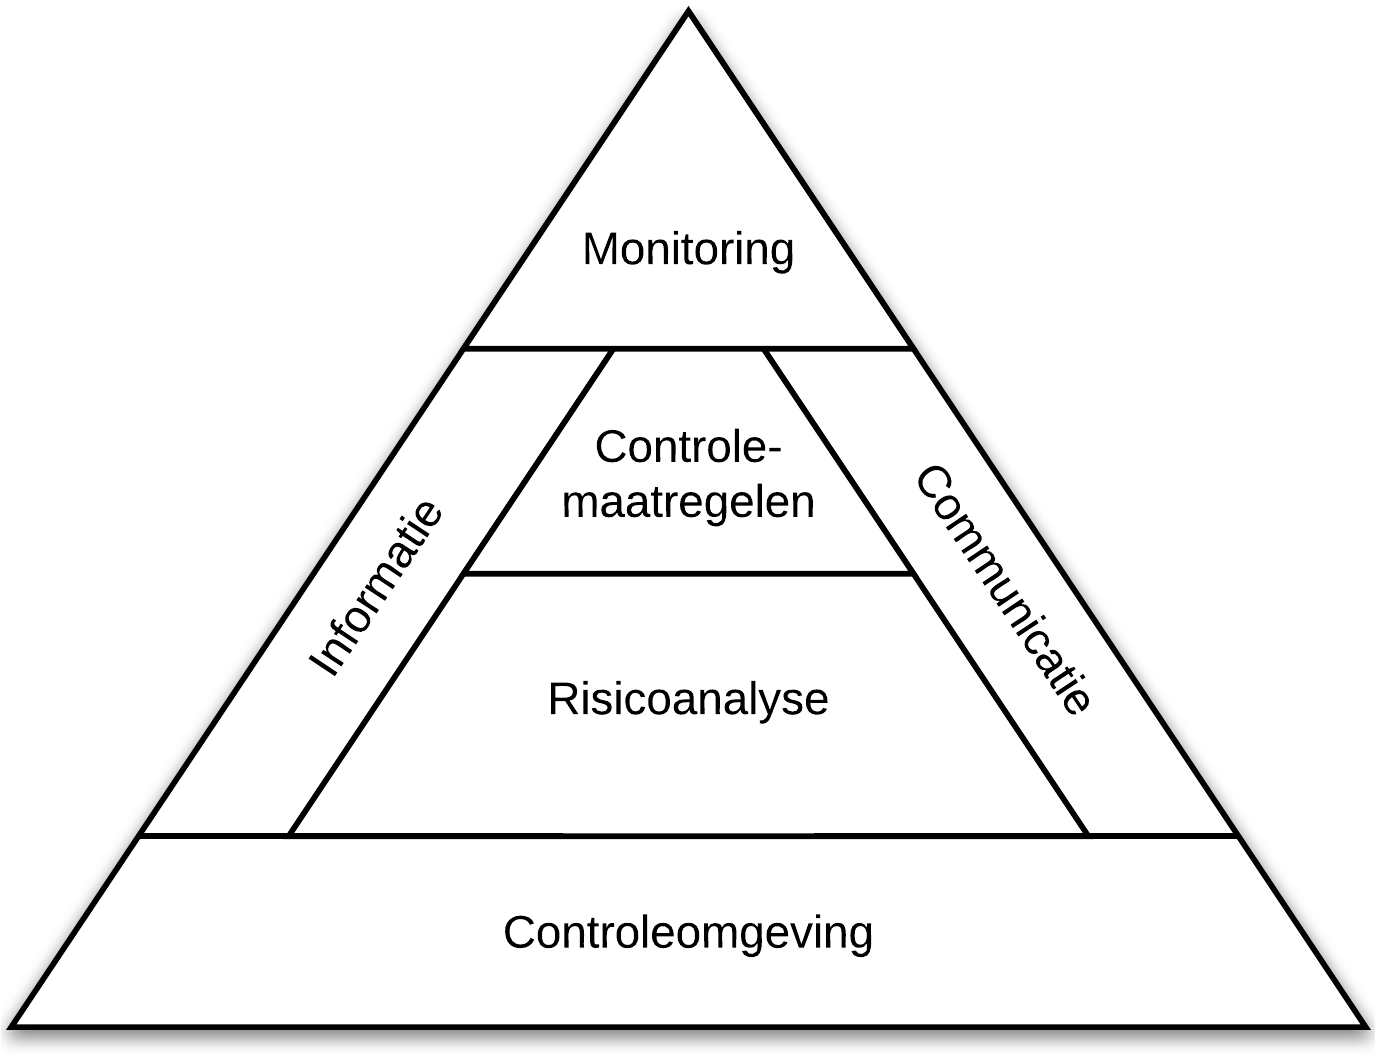
\includegraphics[width=0.6\textwidth]{coso}
    \caption{Het COSO Internal Control Framework \citep{COSOsummery}}
    \label{fig:coso}
\end{figure}

\subsection{Het vakgebied}
Deze onderzoeksopdracht valt onder de noemer 'betrouwbaarheid breed'. Deze is gericht op het inrichten van het interne betrouwbaarheidssysteem in het algemeen. Deze opdracht wordt voornamelijk toegepast bij organisaties die sterk aan het groeien zijn en die graag willen weten of de bestaande interne controlemaatregelen nog voldoende zijn. Een veel voorkomende opdracht hierbij is dat het bestaande AOIB handboek verouderd is. \citep{bivpraktijk}


\newpage
\subsection{Operationalisatie deelvragen}
\begin{enumerate}
    \item Controle-omgeving
        \begin{itemize}
            \item Hoe kan de cultuur van Seafood Connection worden getypeerd?
            \item Wat is de houding van de directie ten opzichte van interne controle?
            \item Wat is de kwaliteit van toezicht op de leiding?
            \item Hoe zijn de economische omstandigheden binnen de branche en de regio? Welke technologische ontwikkelingen hebben een sterke invloed op de branche?
            \item Heeft Seafood Connection een personeelsreglement of code of conduct? Wordt deze genoeg bekend gemaakt bij medewerkers en wordt deze periodiek geëvalueerd?
            \item Welke wetten en regels zijn specifiek voor de branche van Seafood Connection?
            \item Wat is de wijze van belonen van medewerkers?
            \item Wat is de kennis en kunde van de medewerkers ten aanzien van de gestelde strategische doelen en geformuleerde missie?
            \item Is SFC controleplichtig? Speelt dit een rol in organisatorische vormgeving en verslaggeving (mede met het oog op compliance)? Speelt de grootte van de organisatie een rol?
            \item Wie zijn de kernspelers in de geld-goederenbeweging?
        \end{itemize}
    \item Risicoanalyse
        \begin{itemize}
            \item Is er een zekere mate van risicobewustzijn binnen de organisatie?
            \item Welke betrouwbaarheidsrisico's zijn te onderkennen gezien de typologie van Seafood Connection en de waardekringloop? Worden deze risico's herkend in de werkelijkheid?
            \item Welke betrouwbaarheidsrisico's zijn te onderkennen door de jaarrekening te onderzoeken?
            \item Welke betrouwbaarheidsrisico's zijn te onderkennen door de aanwezige processen te onderzoeken? Is er een zeker verband tussen de afdelingen die extra betrouwbaarheidsrisico's met zich meebrengen (bijvoorbeeld de manier waarop wordt omgegaan met het geldmiddelenbeheer)?
        \end{itemize}
    \item Preventieve en repressieve maatregelen van interne controle
        \begin{itemize}
            \item Welke preventieve maatregelen zijn getroffen? (zie tabel \ref{tab:icmaatregelen})
            \item Welke repressieve maatregelen zijn getroffen? (zie tabel \ref{tab:icmaatregelen})
        \end{itemize}
    \item Informatie en communicatie
        \begin{itemize}
            \item Welke informatie is voorhanden aan directie over belangrijke betrouwbaarheids- en bedrijfsrisico's?
            \item Wat is de kwaliteit van de communicatie binnen de organisatie?
            \item Wat is de kwaliteit van de communicatiesystemen binnen de organisatie?
            \item Wordt er voldaan aan de compliance voor externe verslaggeving? 
            %Volgen van NL-GAAP in de externe jaarrekening met betrekking tot verwerking in te kopen / ingekochte vreemde valuta. Wordt nu verwerkt als \textit{niet uit de balans blijkende verplichtingen}, maar er hangt natuurlijk ook een niet uit de balans blijkend recht aan
        \end{itemize}
    \item Monitoring (of: borging)
        \begin{itemize}
            \item Worden de voorschriften en regels met betrekking tot interne betrouwbaarheid nageleefd?
            \item Is het interne betrouwbaarheidssysteem nog steeds actueel en relevant voor de organisatie?
        \end{itemize}
\end{enumerate}


\begin{table}[!h]
    \centering
    \caption{Het stelsel van maatregelen van interne controle \citep{bivpraktijk}}
    \begin{tabular}{l l}
        \toprule
        \textbf{Preventieve maatregelen van IC} & \textbf{Repressieve maatregelen van IC} \\
        \midrule
        Begrotingen, normen, en tarieven & Cijferbeoordeling \\
        Functiescheiding & Verbandscontroles \\
        Procedures en richtlijnen & Detailcontroles \\
        Beveiliging van waarden & Waarneming ter plaatse \\
        Preventieve IT-controls & Repressieve IT-controls \\
        Inrichting van de administratie \\
        \bottomrule
    \end{tabular}
    \label{tab:icmaatregelen}
\end{table}